% Chapter 1

\chapter{Introducción general} % Main chapter title

\label{Chapter1} % Change X to a consecutive number; for referencing this chapter elsewhere, use \ref{ChapterX}


En este capítulo se explica brevemente el marco en el cual se desarrolló el trabajo y se dan las primeras definiciones sobre el equipo construido. 
%----------------------------------------------------------------------------------------
%	SECTION 1
%----------------------------------------------------------------------------------------
\section{Contexto}

El trabajo realizado consistió en la construcción de un equipo comercial \textit{dip coater}, el mismo se desarrolló en el marco de la fundación de la empresa \textit{TECSCI (Technology for Science)}\citep{web_tecsci}.

La empresa tiene como visión ser referente internacional en el desarrollo de equipamiento científico y como misión pretende fabricar productos innovadores de alta calidad. Espera poder dar respuesta a las demandas de laboratorios de investigación, universidades y empresas de base tecnológica nacionales e internacionales.

Como valor agregado se destaca que la empresa adhiere a la filosofía del software y hardware libre \citep{web_oshwa}, por lo tanto, el lector podrá acceder a todo el código fuente del firmware \citep{web_firmware_tecsci}, a los archivos de diseño y fabricación del circuito impreso \citep{web_hardware_tecsci} y a los modelos de piezas mecánicas necesarias para replicar, reparar o adaptar el equipo según sus necesidades.

Las soluciones que propone se orientan a dar respuesta a las problemáticas que se comparten tanto en el mercado local como en el internacional:
\begin{itemize}
\item Elevado precio del equipamiento científico y de su mantenimiento.
\item Contratación exclusiva de servicio técnico asociado al fabricante.
\item Soluciones de software y hardware cerradas que no permiten la adaptación del instrumental a experimentos científicos personalizados.
\end{itemize}


La empresa está incubada en FUNINTEC (Fundación Unsam Innovación y Tecnología) y sus instalaciones se encuentran dentro del Campus Miguelete en la UNSAM ( Universidad Nacional de San Martín). El contrato de incubación le permite contar con un taller mecánico con maquinaria suficiente para la fabricación de  prototipos, con la posibilidad de poder escalarlos hacia una etapa de producción. A continuación se mencionan los recursos mas importantes:
 
\begin{itemize}
\item Torno \textit{CNC (Computer Numerical Control)}.
\item Centro de mecanizado CNC.
\item Torno y fresadora manual.
\item Láser de corte.
\item Cabina de \textit{blasting}
\end{itemize}

En la siguiente figura \ref{fig:taller} se observan los equipos mencionados.

\begin{figure}[htpb]
\centering 
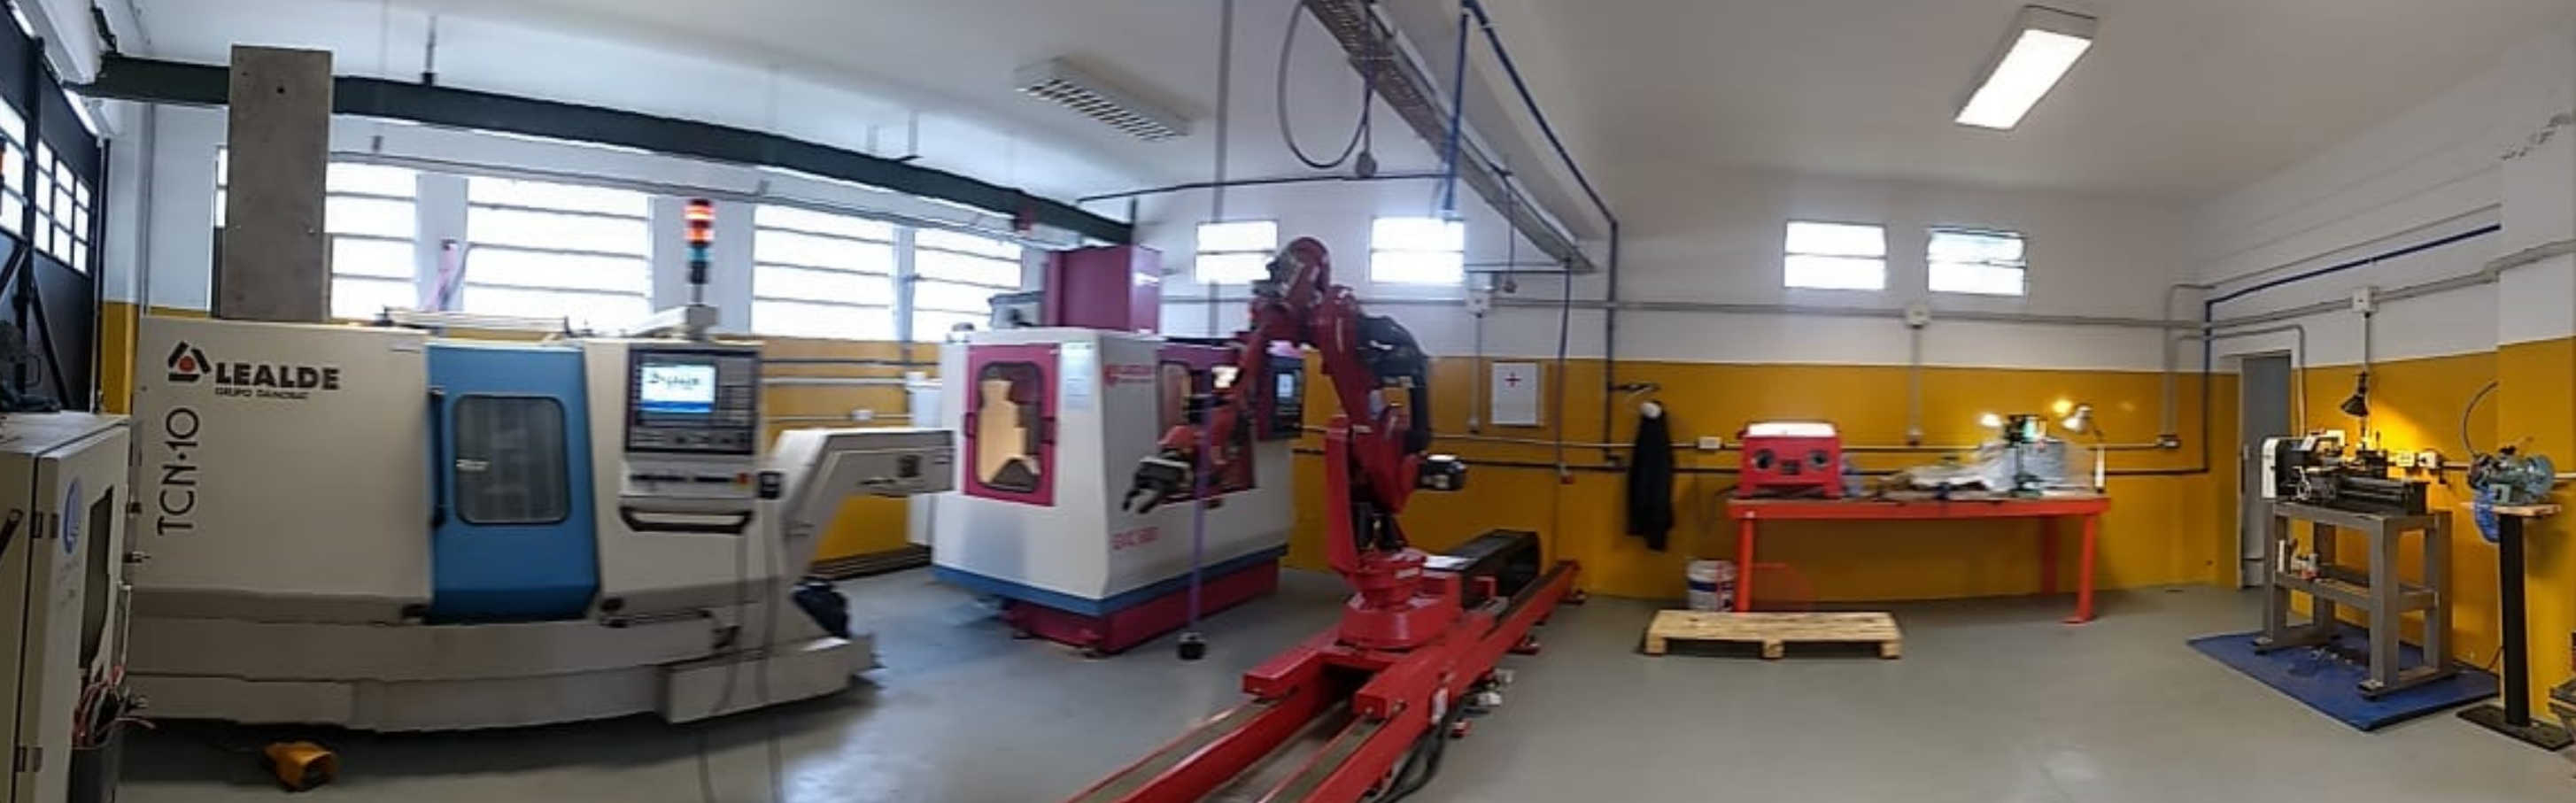
\includegraphics[width=1\textwidth]{./Figures/taller.jpg}
\caption{Centro Tecnológico FUNINTEC.}
\label{fig:taller}
\end{figure}

La empresa también cuenta con un laboratorio de electrónica con equipos para diseño y prototipado electrónico.

%----------------------------------------------------------------------------------------
%	SECTION 2
%----------------------------------------------------------------------------------------
\section{Técnicas de dip coating}

En los laboratorios de investigación aplicados en nanotecnologías existen diferentes equipos para la fabricación de películas delgadas o \textit{thin films}. Las mismas consisten en capas de material de espesores variables, que comúnmente van desde las centenas de nanómetros hasta las decenas de micrómetros y se depositan sobre diferentes superficies.


\textit{Dip coating} es una técnica que se emplea tanto en áreas de I+D (investigación y desarrollo) en la industria, como en la investigación científica en el campo de las nanociencias, se basa en la inmersión y extracción  controlada de un sustrato en una solución química bajo estudio. En la figura \ref{fig:inmersion} se observa una ejecución completa del movimiento desarrollado:


\begin{figure}[htpb]
\centering 
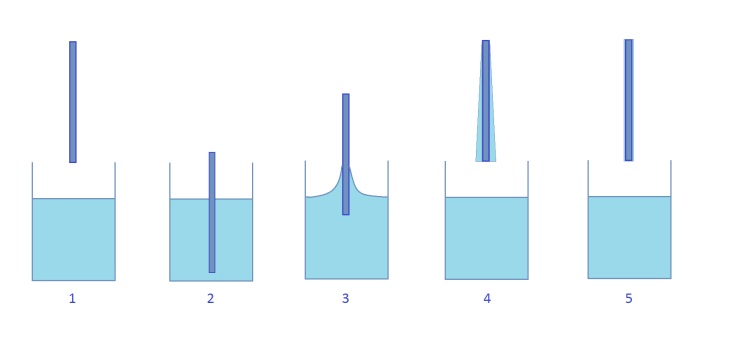
\includegraphics[width=0.85\textwidth]{./Figures/dip-coating.png}
\caption{Proceso completo desarrollado por el equipo \protect\footnotemark.}
\label{fig:inmersion}
\end{figure}
\footnotetext{Imagen tomada de \citep{web_nadetech}}

\begin{enumerate}
\item La muestra desciende a velocidad controlada.
\item La muestra queda sumergida un tiempo establecido por el usuario.	
\item La muestra asciende a velocidad controlada, este es el punto más crítico del experimento, en donde el material queda adherido a la muestra. Se estudiarán en el capítulo \ref{Chapter3} dos modelos matemáticos que explican este fenómeno y se dará una noción mas detallada de las velocidades que caracterizan al proceso.
\item Se extrae toda la muestra.
\item El usuario puede tener interés en volver a repetir el proceso un tiempo después.
\end{enumerate} 
 
La principal característica del equipo es brindarle al usuario la posibilidad de controlar la velocidad y aceleración de inmersión de la muestra, el tiempo de espera que la muestra queda sumergida y la extracción, teniendo la posibilidad de repetir el ciclo según se desee.

Como ejemplo de los resultados que se obtienen aplicando está técnica se observan en la figura \ref{fig:muestras} films de dioxido de titanio \ce{TiO2}. En la imagen A el film se preparó sobre un wafer de silicio y en la imagen B sobre un portaobjeto de vidrio.


\begin{figure}[!htpb]
     \centering
     \begin{subfigure}[b]{0.4\textwidth}
         \centering
         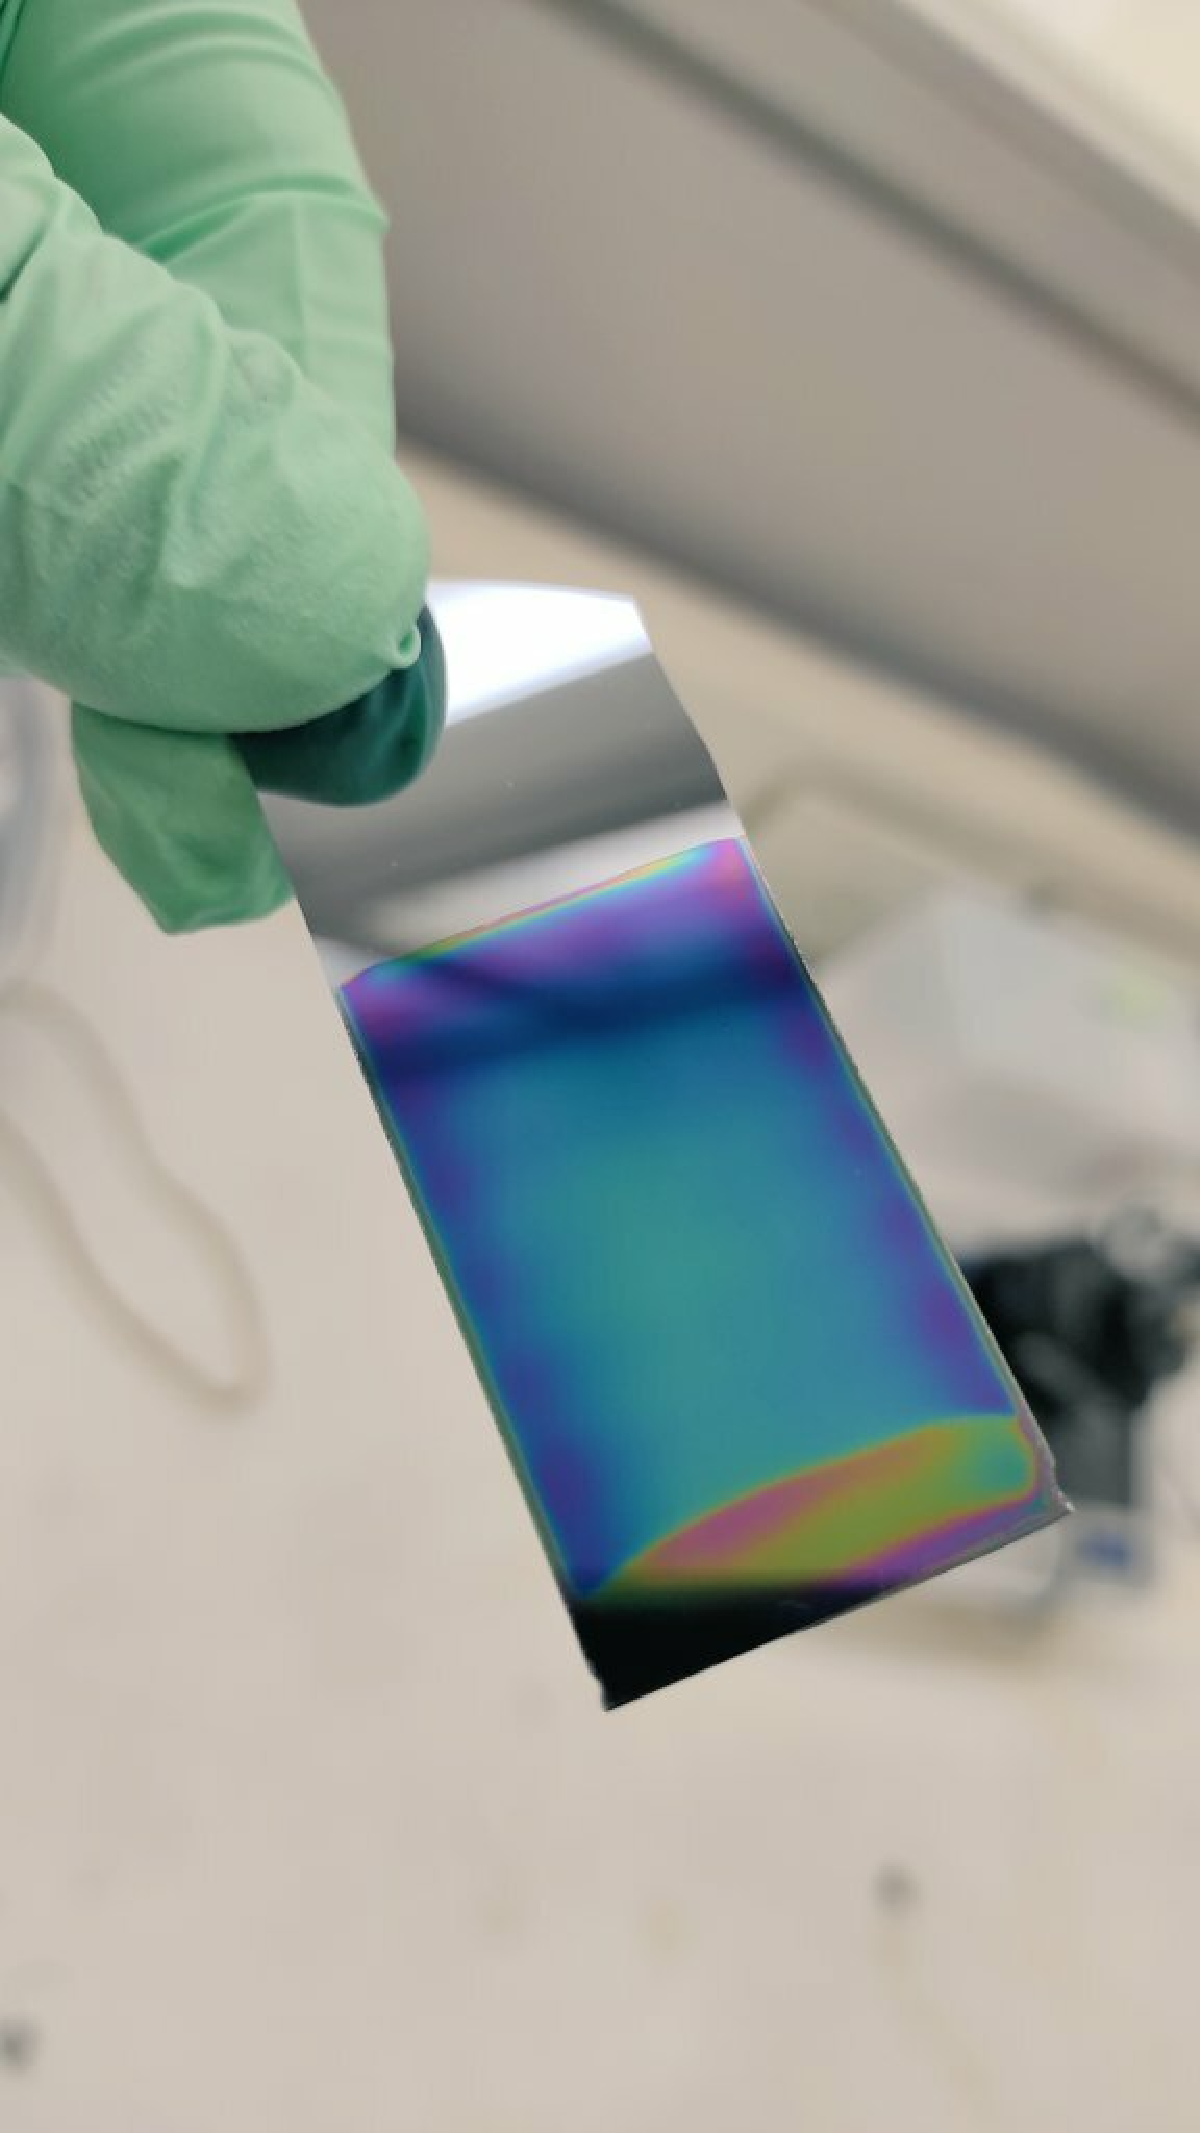
\includegraphics[width=.5\textwidth]{./Figures/muestra_1.pdf}
         \caption{Film sobre wafer de silicio.}
         \label{fig:muestra_1}
     \end{subfigure}
     \hfill
     \begin{subfigure}[b]{0.4\textwidth}
         \centering
         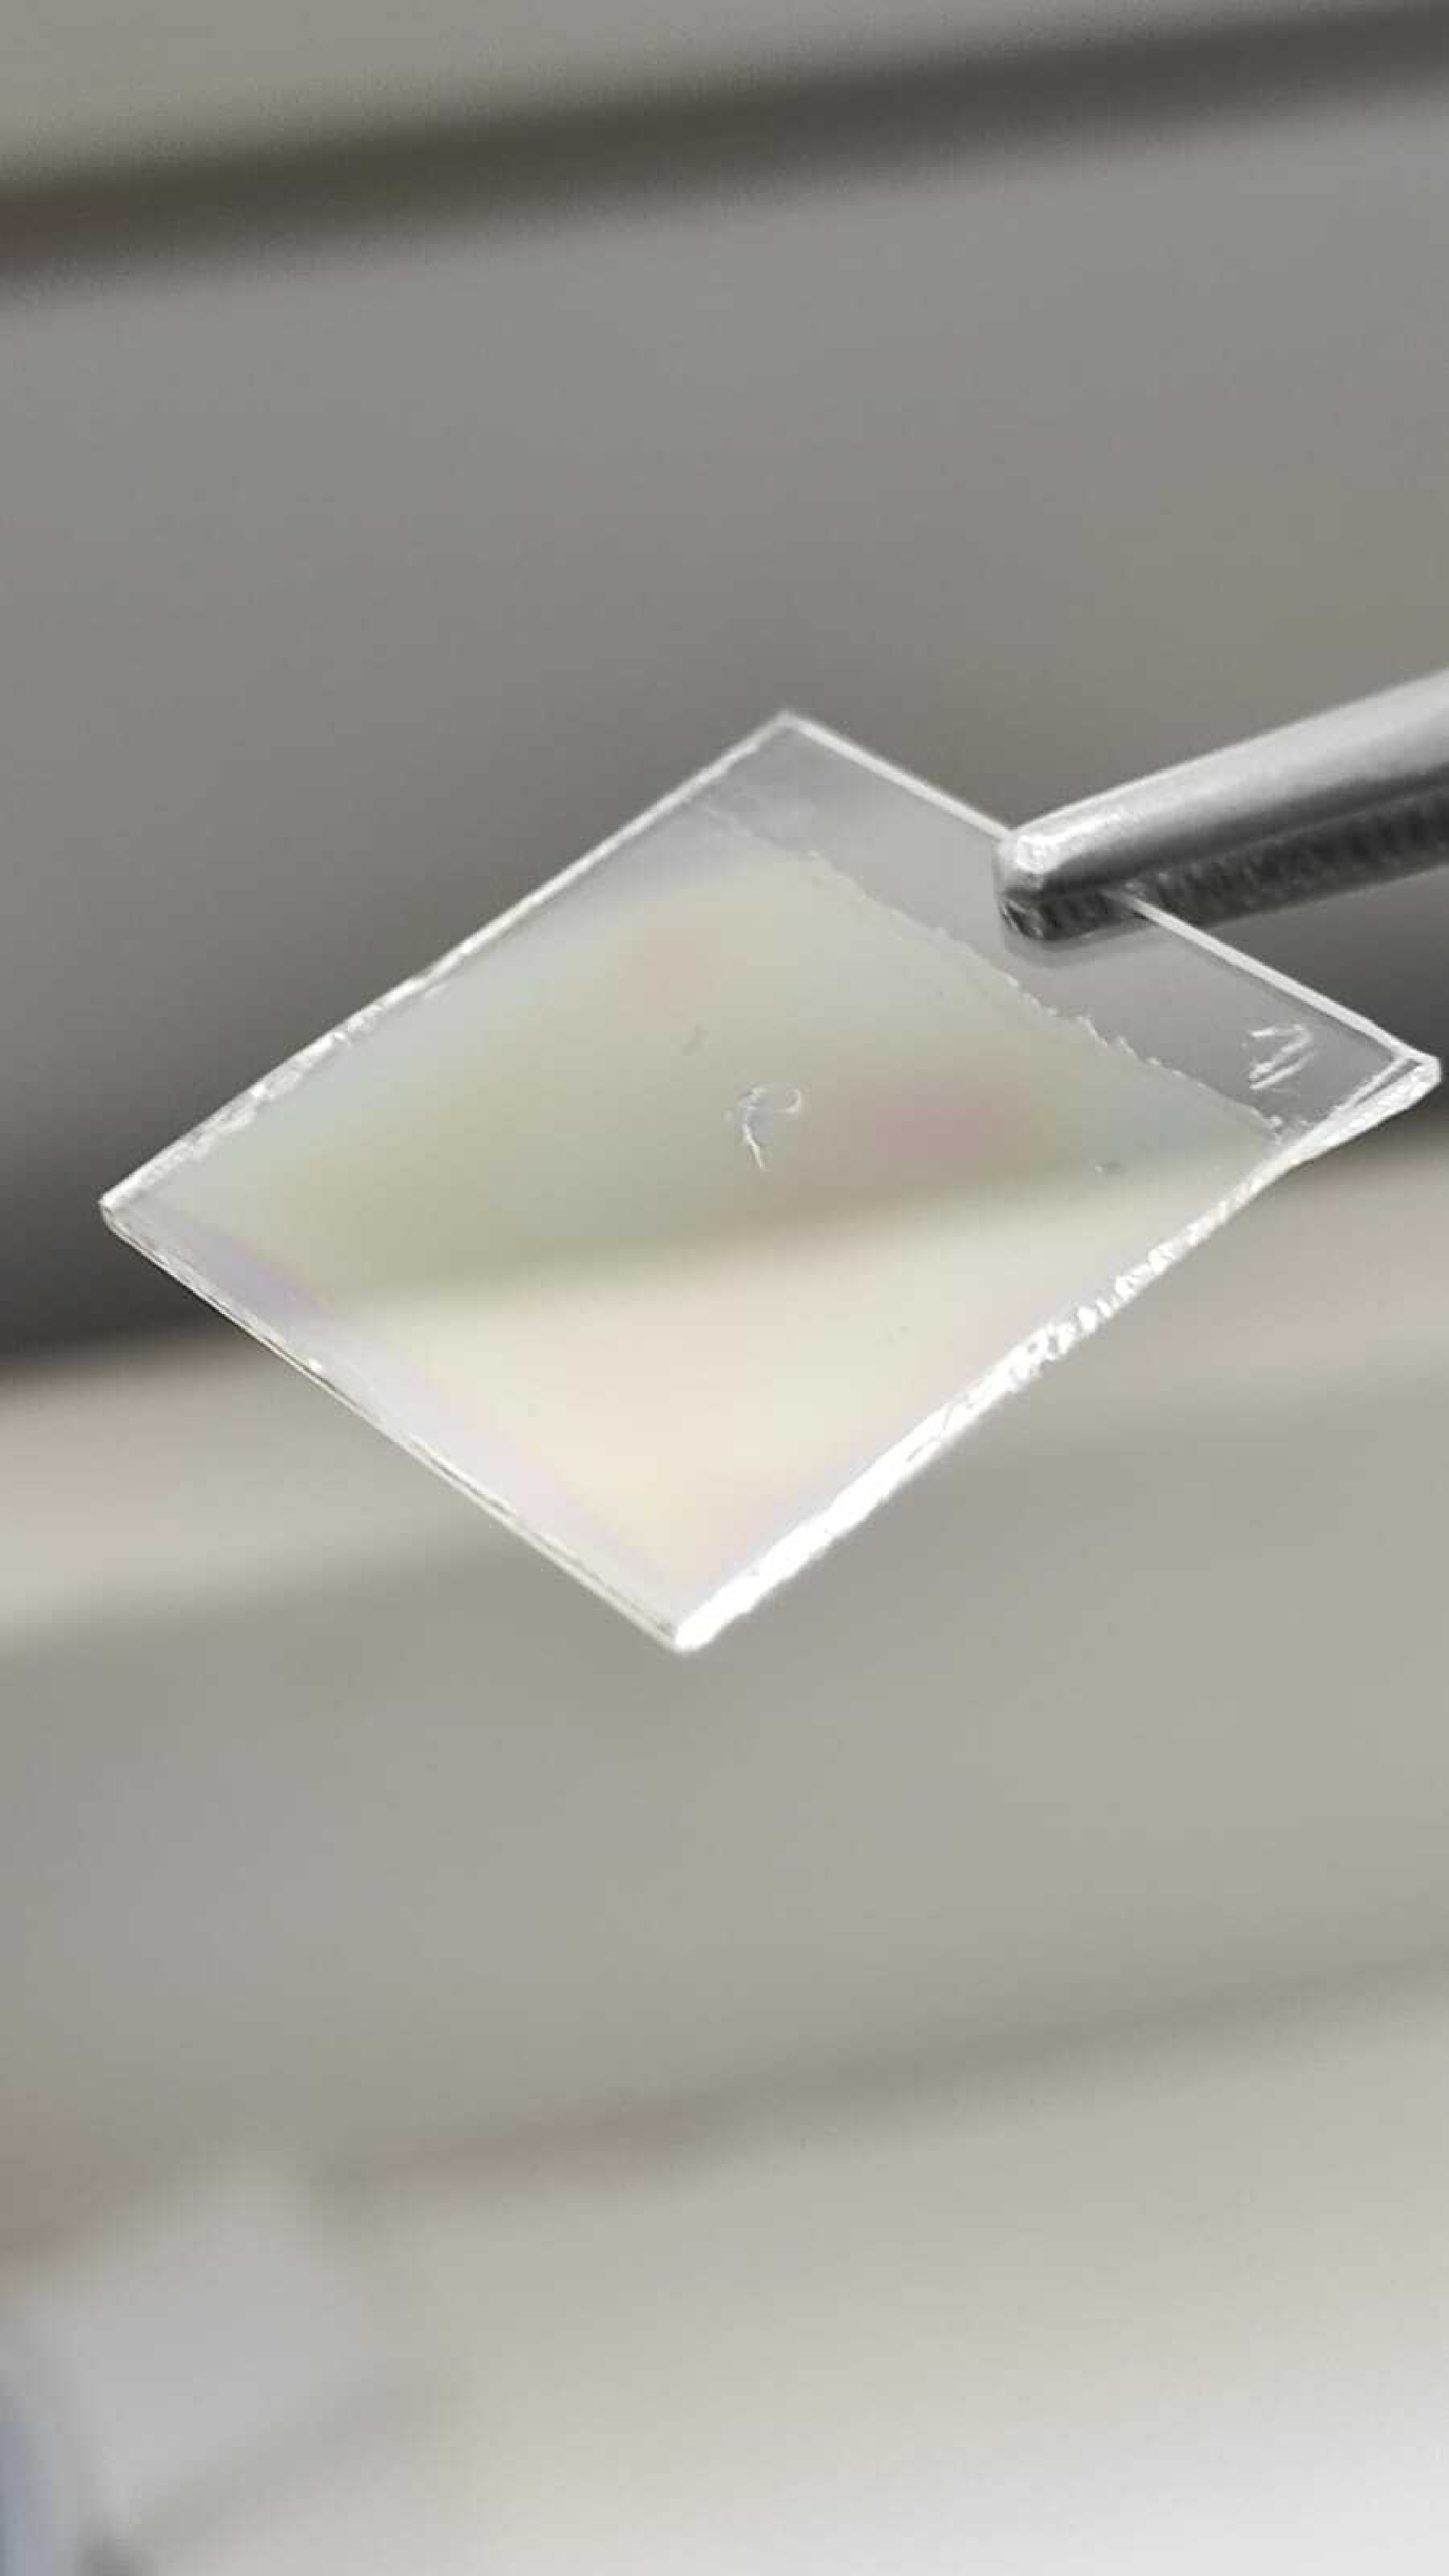
\includegraphics[width=.5\textwidth]{./Figures/muestra_2.pdf}
         \caption{Film sobre portaobjeto.}
         \label{fig:muestra_"}
     \end{subfigure}
     \hfill
        \caption{Films de dioxido de titanio \ce{TiO2} \protect\footnotemark.}
        \label{fig:muestras}
\end{figure}

\footnotetext{Imagen tomada en los laboratorios del Instituto de Nanosistemas de la UNSAM.}


Cabe destacar que los espesores de capa logrados en este experimento fueron de entre \SI{180}{nm} y \SI{200}{nm}, con velocidades de inmersión y extracción configuradas en \SI{180}{mm/min}. Valores de velocidad similares deberán estar contemplados en el desarrollo del presente equipo dip coater.

Luego de un proceso dip coating, dependiendo del tipo de muestra que se genere, es necesario realizar tratamientos térmicos para finalizar el proceso. Los mismos se realizan con otro tipo de equipos y no forman parte del trabajo realizado.
 
\label{sec:dip coating}

%----------------------------------------------------------------------------------------
%	SECTION 3
%----------------------------------------------------------------------------------------
\section{Dip coaters en el mercado}
\label{sec:mercado}
Existen diferentes fabricantes a nivel internacional que comercializan este tipo de equipos, pero ninguno a nivel local. Se presentan a continuación algunos productos de las empresas internacionales con mayor reconocimiento en el ámbito de las nanociencias. 

Se puede observar en la figura \ref{fig:dip_kibron} el equipo de la empresa Kibron \citep{2_web_kibron}.

\begin{figure}[htbp]
	\centering
	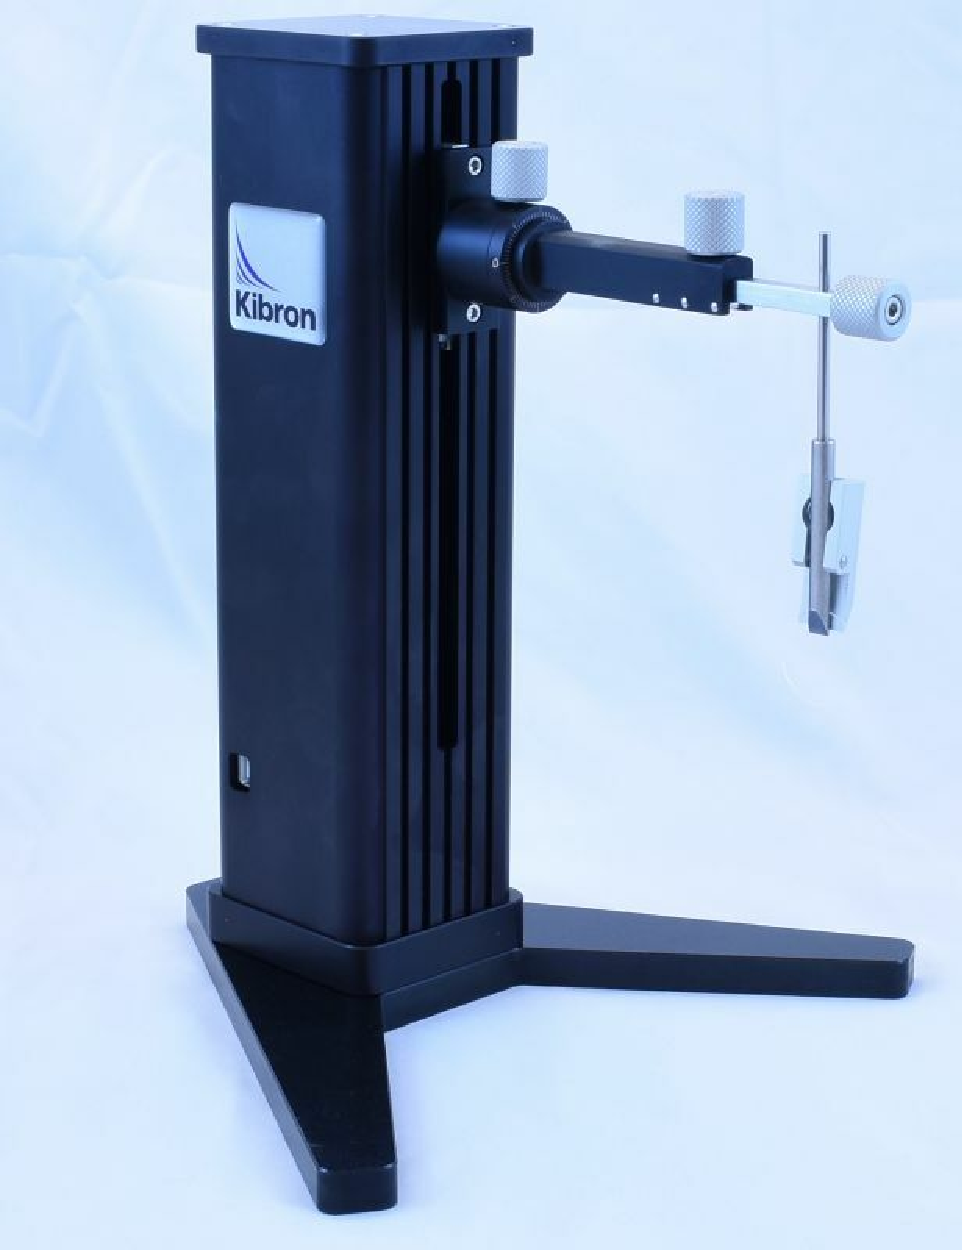
\includegraphics[width=.25\textwidth]{./Figures/kibron.pdf}
	\caption{Equipo de la empresa Kibron.}
	\label{fig:dip_kibron}
\end{figure}

En la figura \ref{fig:equipos_biolin} se observan los equipos de la empresa Biolin Scientific  \citep{1_web_biolin}, un equipo simple y otro con mayor funcionalidad. Si bien ambos controlan con exactitud la velocidad de inmersión y extracción, el último agrega una funcionalidad extra, que a través de una rotación en la base da la posibilidad de cambiar de manera automática y secuencial las soluciones donde se realizan las inmersiones. Ambos equipos necesitan estar conectados a una computadora corriendo un software para poder ser accionados.

\begin{figure}[!htpb]
     \centering
     \begin{subfigure}[b]{0.4\textwidth}
         \centering
         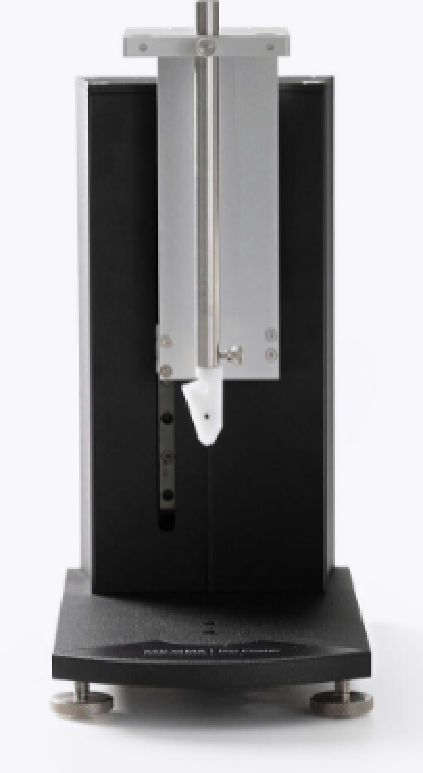
\includegraphics[width=.45\textwidth]{./Figures/dip_biolin.pdf}
         \caption{Equipo simple.}
         \label{fig:dip_biolin}
     \end{subfigure}
     \hfill
     \begin{subfigure}[b]{0.4\textwidth}
         \centering
         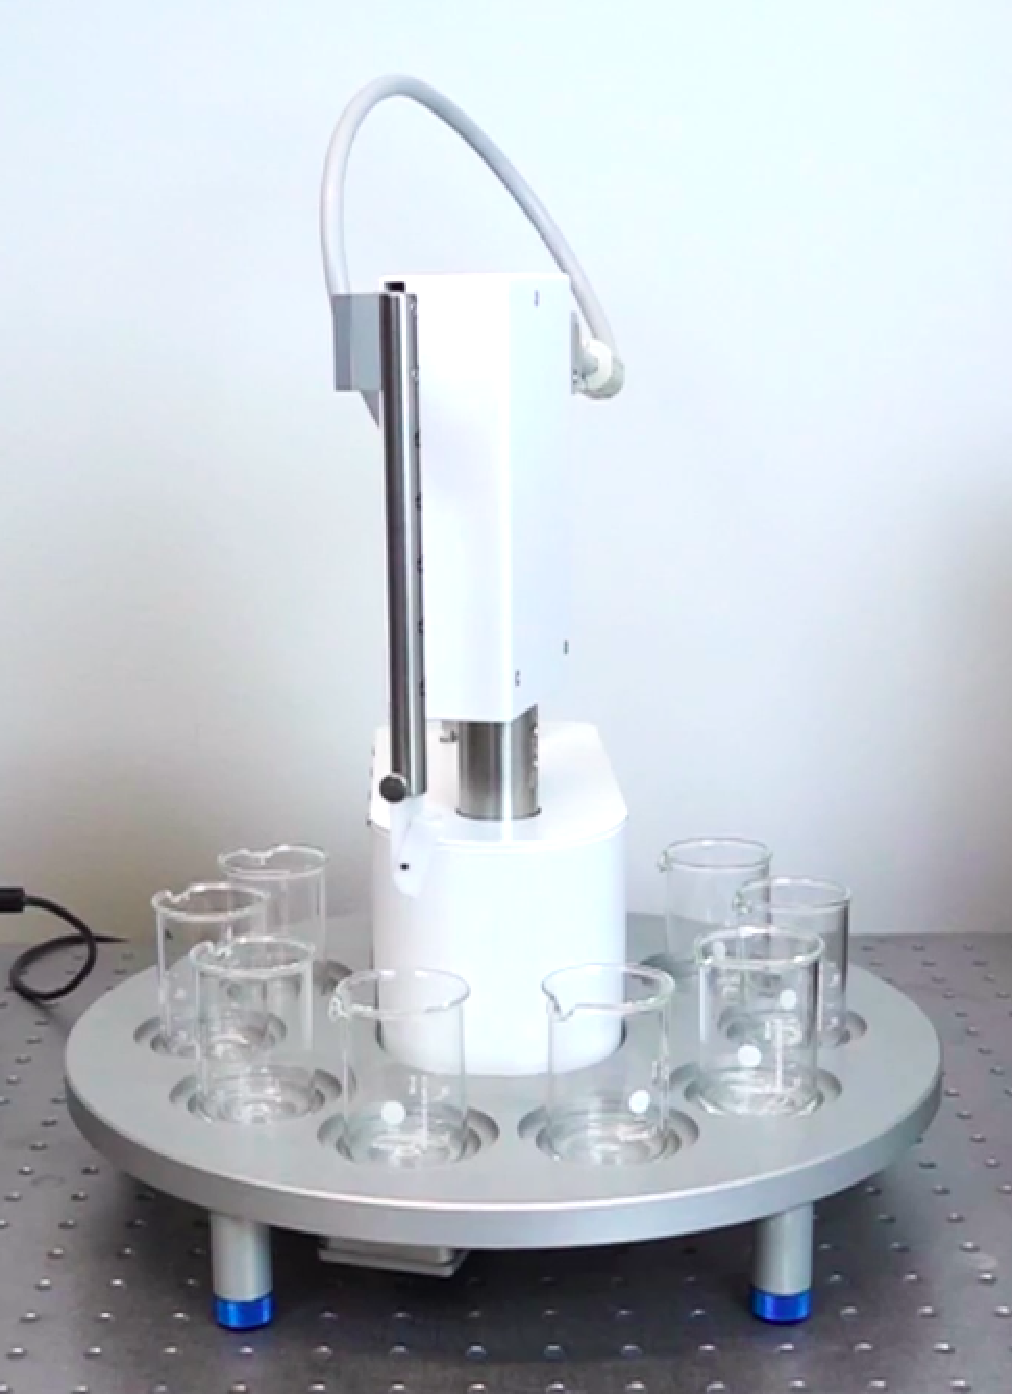
\includegraphics[width=.65\textwidth]{./Figures/dip_biolin_2.pdf}
         \caption{Equipo avanzado.}
         \label{fig:dip_biolin_2}
     \end{subfigure}
     \hfill
        \caption{Equipos de la empresa Biolin Scientific.}
        \label{fig:equipos_biolin}
\end{figure}

Por último se presenta el equipo de la empresa Bungard \citep{6_web_bungard}, que puede observarse en la figura \ref{fig:dip_bungard}.
Este equipo a diferencia de los otros cuenta con un display LCD y botonera, lo que permite al usuario realizar una configuración a pie de máquina.

\begin{figure}[htbp]
	\centering
	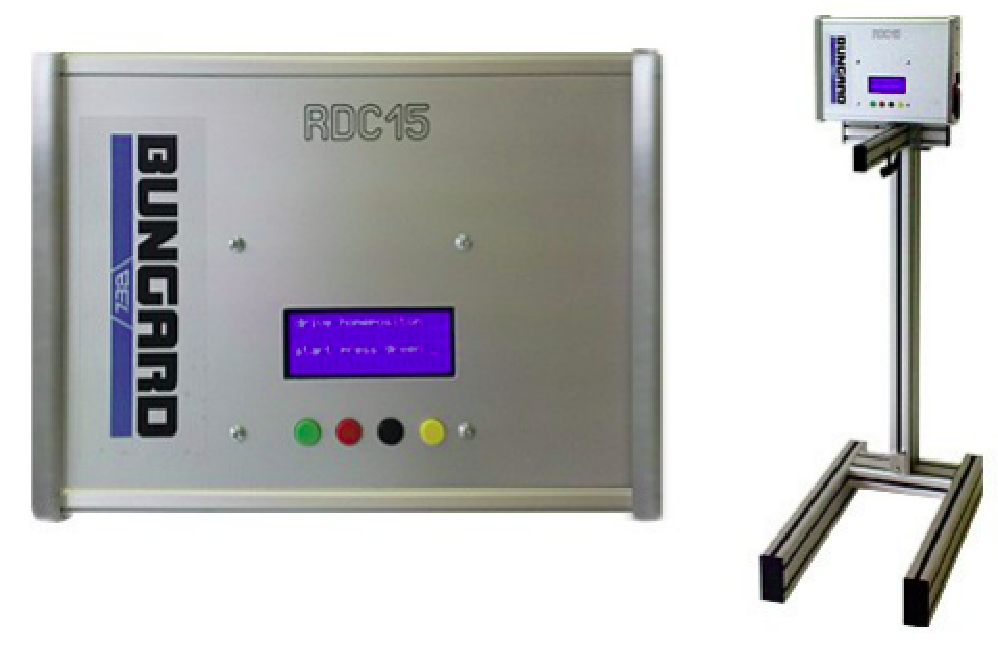
\includegraphics[width=.45\textwidth]{./Figures/6_bungard.pdf}
	\caption{Equipo de la empresa Bungard.}
	\label{fig:dip_bungard}
\end{figure}

A continuación se presenta la tabla \ref{tab:equipos_competencia} en donde se comparan las especificaciones técnicas que los caracterizan. 

\begin{table}[h]
	\centering
	\caption[Dip coaters en el mercado]{Especificaciones técnicas de otros equipos.}
	\begin{tabular}{l c c c c}    
		\toprule
		\textbf{Equipo} 	 & \textbf{Recorrido}  & \parbox{2cm} {\textbf{Velocidad (mm/min)}}  & \parbox{2cm}{\textbf{Aceleración (m/min2)}}  & \textbf{Interface} \\
		\midrule
		Bio Single Vessel M	& 300 mm 	& 1    - 1000   & no & PC 							\\		
		Bio Multiplie Vessel		& 70  mm	& 0.1  - 108 	& no & PC					\\
		Kibron LayerX				& 134 mm	& 0.06 - 300	& no & PC					\\
		Bungard						& 600 mm	& 30 - 10000	& no & Display LCD		\\
		Ossila \citep{4_web_ossila}					& 100 mm	& 0.6  - 3000	& no & PC		\\
		Holmarc	\citep{5_web_holmarc}					& 100 mm	& 1.08 - 540	& no & PC		\\
		\bottomrule
		\hline
	\end{tabular}
	\label{tab:equipos_competencia}
\end{table}


Se realizaron consultas a investigadores científicos, los cuales indicaron que el rango de velocidades más utilizado para la generación de \textit{films} es el de [1 a 200 \si{\milli\meter\per\minute}]. Se destaca que la mayoría de los equipos presentados cumplen con dicha indicación.

Del análisis de la tabla se pueden extraer algunas conclusiones: ninguno de los equipos permite al usuario tener control sobre la aceleración en los movimientos de inmersión y extracción de muestra, la mayoría  de los equipos depende de una comunicación USB-SERIAL con una computadora, ninguna de las empresas adhiere a los principios del software y hardware libre.  

%----------------------------------------------------------------------------------------
%	SECTION 4
%----------------------------------------------------------------------------------------

\section{Objetivos y alcance}

\subsection{Objetivos}

El objetivo de este trabajo fue diseñar y fabricar el primer equipo comercial de la empresa TECSCI, con la perspectiva a futuro de ampliar la gama ofrecida de equipos de laboratorio para la investigación científica.

También es parte de los objetivos fundamentales que el equipo desarrollado incorpore mejoras respecto a sus competidores. Se planteará en los siguientes capítulos un estudio sobre el control de movimientos elegido y se presentará un sistema moderno de configuración de equipo. 

\subsection{Alcance}

El presente trabajo abarca la presentación de un MVP (Producto Mínimo Viable) de equipo dip coater. 


El trabajo realizado incluye:

\begin{itemize}
\item Driver de motor provisto por el fabricante TRINAMIC \citep{3_web_trinamic}.
\item Diseño de hardware con software de diseño KICAD \citep{web_kicad}.
\item Fabricación de placa electrónica y montaje de componentes.
\item Diseño y fabricación de partes mecánicas a través del mecanizado de aluminio.
\item Incorporación de pantalla táctil para configuración y uso del equipo.
\end{itemize}



El trabajo no incluye:

\begin{itemize}
\item Desarrollo de hardware con fuente de alimentación incorporada.
\item Programación de la interfaz gráfica con el software de diseño provisto por
el fabricante de la pantalla.
\item Control del entorno con cámara de humedad.
\end{itemize}


